\documentclass[times, utf8, zavrsni]{fer}
\usepackage{booktabs}
\usepackage{graphicx}
% -- Loading the code block package:
\usepackage{listings}% -- Basic formatting
\setlength{\parindent}{8pt}
\usepackage{indentfirst}% -- Defining colors:
\usepackage[dvipsnames]{xcolor}
\usepackage{caption}
\definecolor{codegreen}{rgb}{0,0.6,0}
\definecolor{codegray}{rgb}{0.5,0.5,0.5}
\definecolor{codepurple}{rgb}{0.58,0,0.82}
\definecolor{backcolour}{rgb}{1,1,1}% Definig a custom style:
\lstdefinestyle{mystyle}{
    backgroundcolor=\color{backcolour},   
    commentstyle=\color{codepurple},
    keywordstyle=\color{NavyBlue},
    numberstyle=\tiny\color{codegray},
    stringstyle=\color{codepurple},
    basicstyle=\ttfamily\footnotesize\bfseries,
    breakatwhitespace=false,         
    breaklines=true,                 
    captionpos=t,                    
    keepspaces=true,                 
    numbers=left,                    
    numbersep=5pt,                  
    showspaces=false,                
    showstringspaces=false,
    showtabs=false,                  
    tabsize=2
}% -- Setting up the custom style:
\lstset{style=mystyle}
\bibliography{literatura.bib}
\bibliographystyle{fer}
\definecolor{light-gray}{gray}{0.95}
\newcommand{\code}[1]{\colorbox{light-gray}{\texttt{#1}}}
\newcommand{\source}[1]{\caption*{Source: {#1}} }


\begin{document}

% TODO: Navedite broj rada.
\thesisnumber{000}

% TODO: Navedite naslov rada.
\title{Klasifikacija prometnih znakova}

% TODO: Navedite vaše ime i prezime.
\author{Matija Pavlović}

\maketitle

% Ispis stranice s napomenom o umetanju izvornika rada. Uklonite naredbu \izvornik ako želite izbaciti tu stranicu.
\izvornik

% Dodavanje zahvale ili prazne stranice. Ako ne želite dodati zahvalu, naredbu ostavite radi prazne stranice.
\zahvala{}

\tableofcontents

\chapter{Uvod}
Razvoj tehnologije u automobilskoj industriji u stopu prate i sve veći zahtjevi tržišta za novim sigurnosnim značajkama te značajkama koje doprinose udobnosti korištenja vozila. Novi modeli vozila tako postaju opremljeni značajnim brojem senzora na vanjskoj strani vozila i značajnim brojem ekrana i signalnih lampica u unutrašnjosti vozila. Kada sjednemo za upravljač novijih vozila sve češće možemo primijetiti da nas vozilo upozorava na prometne znakove, primjerice ograničenja brzine, zabrane pretjecanja, znakove obaveznog zaustavljanja itd. Razmotrimo li i činjenicu da ubrzano raste i broj vozila s određenim stupnjem autonomije pri vožnji postaje jasno da su sustavi koji u stvarnom vremenu detektiraju i klasificiraju prometne znakove postali izrazito važni u razvoju novih modela vozila. Cilj ovog završnog rada je demonstracija rada jednog takvog sustava uz detaljni opis primjene, problema s kojima se sustav može suočavati u stvarnim okolnostima, te opis implementacije sustava. U sklopu rada ću razviti model strojnog učenja temeljen na dubokoj konvolucijskoj mreži, obraditi skup podataka za treniranje i testiranje modela, te programski kod koji će koristiti kameru prijenosnog računala kako bi klasificirao prometne znakove.

\chapter{Pregled postojeće literature}
Klasifikacija prometnih znakova nije nov pojam u području računarske znanosti i specifičnije području računalnog vida. Shodno tome postoji velik broj znanstvenih radova koji se bave tom problematikom.
Većina pristupa problemu klasifikacije se bazira na pristupu usmjerenom na prepoznavanje boja i oblika.\citep{6033494}
\chapter{Metodologija rada}
U poglavlju metodologija rada opisati ću metode pri izradi projekta od razine prikupljanja i prilagodbe podataka za treniranje modela strojnog učenja, kreiranje samog modela, treniranje modela te naposlijetku i izradu testne aplikacije kojom se demonstrira rad sustava.
\pagebreak
\section{Prikupljanje podataka za treniranje}
Skup podataka za treniranje odnosno
\emph{Dataset} korišten u ovom radu je je preuzet iz elektronske arhive istraživačkih radova Sveučilišta u Kopenhagenu(Electronic Research Data Archive).
\emph{Dataset} je dio \emph{German Traffic Sign Recognition Benchmark}-a (GTSRB), a kreirali su ga Johannes Stallkamp, Marc Schlipsing, Jan Salmen, Christian Igel.
Navedeni skup podataka se sastoji od 34799 slika, raspodijeljenih u 43 razreda koji predstavljaju 43 različita prometna znaka.

\begin{figure}[h!]
  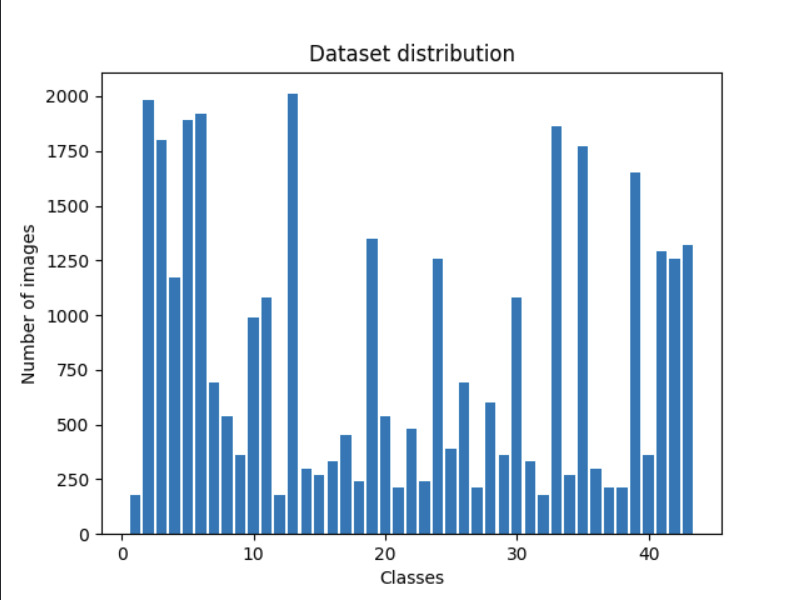
\includegraphics[width=\linewidth,trim=4 4 4 4,clip]{images/distribution.jpeg}
  \caption{Raspodijela dataseta po razredima.}
\end{figure}
\pagebreak
\section{Pretprocesiranje}
Pretprocesiranje ulaznog skupa podataka obavlja se pomoću sljedećeg bloka programskog koda:
\begin{lstlisting}[language=Python]
import cv2


def preprocess(image):
    image = cv2.cvtColor(image, cv2.COLOR_BGR2GRAY)
    image = cv2.equalizeHist(image)
    image = image / 255
    return image
    return data_gen
\end{lstlisting}

S obzirom da za prepoznavanje zadanog skupa prometnih znakova nije potrebna informacija o boji, svaka ulazna slika se pretvara u \emph{grayscale}.
Također kako bi \emph{dataset} bio što iskoristiviji, slikama se povećava kontrast tehnikom histogramskog izjednačavanja. Metoda izjednačavanja histograma (HE) je široko korištena tehnika pretprocesiranja slike i svrstava se u kategoriju korekcija svjetline. 
Primjeri primjene HE su poboljšanje medicinskih slika, znanstvenih fotografija, povijesnih slika i sonarskih slika. Histogramsko izjednačavanje se također koristi i za poboljšanje kontrasta slike u digitalnim slikama. 
Navedeni učinci se postižu učinkovitim distribuiranjem najčešćih vrijednosti intenziteta. To omogućuje da povećamo kontrast na lokalnim dijelovima slike s lošim kontrastom.\citep{9642082}
Tehnikom histogramskog izjednačavanja se efektivno proširuje raspon vrijednosti intenziteta s ciljem povećanja kontrasta. Ova tehnika se često koristi i na slikama koje su imale loše osvijetljenje.
Naposlijetku vrijednosti svakog piksela slike se normaliziraju na vrijednost iz skupa [0, 1]. Navedenim postupcima pretprocesiranja se pospješuje brzina i učinkovitost treniranja modela.
\begin{figure}[h!]
  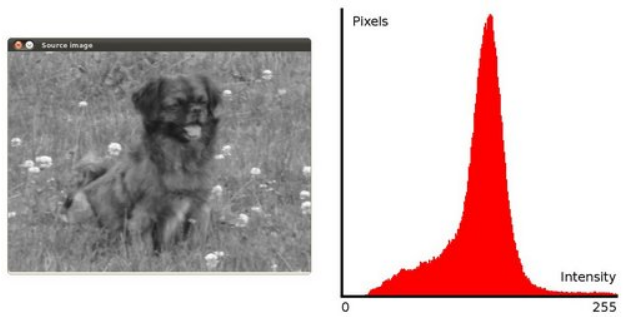
\includegraphics[width=\linewidth,trim=4 4 4 4,clip]{images/hist1.png}
  \caption{Primjer slike prije histogramskog izjednačavanja i odgovrajući histogram.}
  \source{\url{https://docs.opencv.org/3.4/d4/d1b/tutorial_histogram_equalization.html}}
\end{figure}
\begin{figure}[h!]
  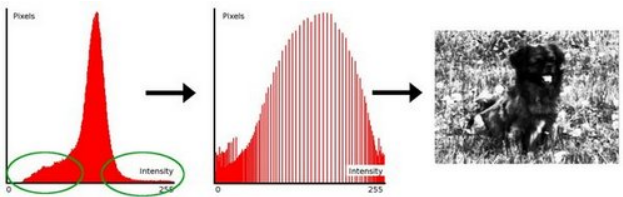
\includegraphics[width=\linewidth,trim=4 4 4 4,clip]{images/hist2.png}
  \caption{Primjer slike nakon histogramskog izjednačavanja i odgovrajući histogram.}
  \source{\url{https://docs.opencv.org/3.4/d4/d1b/tutorial_histogram_equalization.html}}
\end{figure}
\pagebreak
\clearpage
\section{Augmentacija skupa podataka}
Kako bi iskoristivost skupa podataka za treniranje bila maksimizirana korištena je augmentacija nad ulaznim skupom.
Augmentacija se provodi u sljedećem bloku programskog koda:
\\
\begin{lstlisting}[language=Python]
from keras.preprocessing.image import ImageDataGenerator


def augment():
    data_gen = ImageDataGenerator(width_shift_range=0.1,
                                  height_shift_range=0.1,
                                  zoom_range=0.2,
                                  shear_range=0.1,
                                  rotation_range=10)
    return data_gen
\end{lstlisting}

Gore prikazana funkcija koristi \code{ImageDataGenerator} funkciju iz
\\
\code{keras.preprocessing.image} modula. Uz navedene argumente ova metoda proširuje \emph{dataset} tako što svaku sliku
\begin{itemize}
	\item  Nasumično pomiče horizontalno uz maksimalni faktor od 10\% širine slike
	\item  Nasumično pomiče vertikalno uz maksimalni faktor od 10\% visine slike
	\item Uvečava sliku u rasponu od 0\% do 20\%
	\item  Posmiče slike uz maksimalni kut posmaka od 10\textdegree 
	\item  Rotira sliku uz maksimalni kut rotacije od 10\textdegree
\end{itemize}
\begin{figure}[h!]
  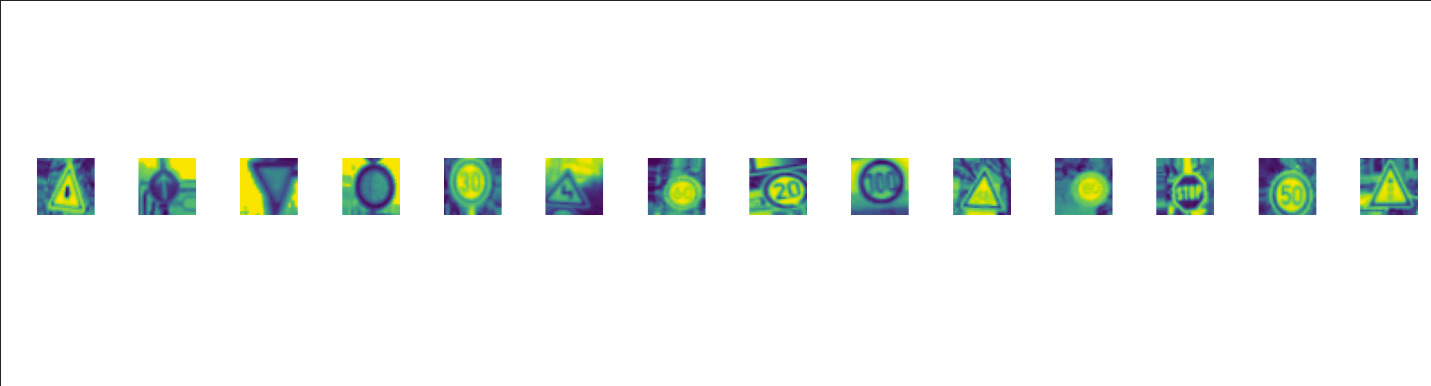
\includegraphics[width=\linewidth,trim=4 4 4 4,clip]{images/image-augmentation.jpeg}
  \caption{Prikaz augmentiranih slika.}
\end{figure}

\section{Treniranje modela}
Model strojnog učenja korišten za izradu ovog rada zasniva se na Keras API-u.
Sastoji se od jedanaest slojeva i reprezentiran je sljedećim isječkom Python koda:
\begin{lstlisting}[language=Python]
from keras.models import Sequential
from keras.layers import Dense
from keras.layers import Dropout, Flatten
from keras.layers.convolutional import Conv2D, MaxPooling2D


def learning_model(classes_len):

    model = Sequential()
    model.add((Conv2D(60, (5, 5), input_shape=(32, 32, 1), activation='relu')))
    model.add((Conv2D(60, (5, 5), activation='relu')))
    model.add(MaxPooling2D(pool_size=(2, 2)))

    model.add((Conv2D(30, (2, 2), activation='relu')))
    model.add((Conv2D(30, (2, 2), activation='relu')))
    model.add(MaxPooling2D(pool_size=(2, 2)))
    model.add(Dropout(0.5))

    model.add(Flatten())
    model.add(Dense(500, activation='relu'))
    model.add(Dropout(0.5))
    model.add(Dense(classes_len, activation='softmax'))

    model.compile(optimizer='adam', loss='categorical_crossentropy', metrics=['accuracy'])
    return model
\end{lstlisting}

Prvi sloj je Conv2D sloj od 60 filtera veličine 5x5 piksela sloj koji prima ulaz oblika 32 piksela visine, 32 piksela širine i 1 piksel dubine jer se radi o \emph{grayscale} slici.
Konvolucijski slojevi neuronske mreže povezuju uzorke na manjim lokalnim regijama sloja s uzorcima koji se pojavljuju na korespondirajućim regijama iz viših slojeva čime se eliminira potreba za stvaranjem potpune povezanosti među slojevima. \citep{8308186}
Korištenjem nekolicine pojednostavljenja konvolucijski slojevi smanjuju broj stvorenih veza i za nekoliko redova veličine.\citep{turner2014lecture}
Sloj koristi ReLU aktivaciju definiranu formulom: \begin{align*} &ReLU(x)= max(0,x)\\ &\frac{d}{dx}(x)\ = \{1\ if\ x>0;\ 0\ otherwise\} \end{align*}
Glavna prednost ove aktivacije je što za ulaz 0, uvijek vraća 0, što nije slučaj kod nekih zasićenih funkcija poput \emph{tanh} i \emph{sigmoid} funkcija. Ovakvo ponašanje može naštetiti treniranju modela.
Drugi, četvrti i peti slojevi modela imaju identičnu zadaću kao i prvi te se stoga ne razmatraju detaljnije.
Treći sloj

Model koristi optimizator Adam...
\pagebreak
\section{Testna aplikacija}
Kako bi se testirala učinkovitost modela, razvijena je jednostavna testna skiripta u programskom jeziku Python. Skripta uključuje  \emph{web-kameru} računala, učitava istrenirani model te povezuje naziv svakog razreda s njegovim indeksom pomoću riječnika.
\\Primjerice:
\begin{lstlisting}[language=Python]
class_names = {
    0: 'Speed Limit 20 km/h',
    1: 'Speed Limit 30 km/h',
    ...
}
\end{lstlisting}

Zatim u beskonačnoj petlji učitava sliku s \emph{web-kamere}, pretprocesira tu sliku, vrši predikciju pomoću istreniranog modela. Ukoliko je vjerojatnost s kojom je model predvidio da se na slici nalazi neki znak veća od unaprijed zadanog praga na zaslonu se ispisuje naziv
znaka te vjerojatnost s kojom model klasificira sliku znaka u pretpostavljeni razred. Naprotiv, ukoliko je vjerojatnost niža od zadanog praga ispisuje se samo prikladna poruka da model ne prepoznaje znak na slici.
\\Uz jasna ograničenja koje ovaj model testne aplikacije posjeduje (nedostatak grafičkog sučelja, uporaba ugrađene kamere umjesto zasebne kamere ili senzora), aplikacija ipak može poslužiti kao kvalitetni pokazatelj učinkovitosti i brzine kojom model vrši predikcije i daje finalni rezultat. 
%TODO: slika izgleda ispisa

\chapter{Rezultati}

\chapter{Budući rad}
Budući rad na ovom problemu bi uključivao implementaciju detekcije prometnih znakova na slici kako bi cjelokupni sustav bio što iskoristiviji u stvarnom svijetu. Nužno bi bilo uvesti i neku vrstu dediciranog senzora ili kamere koja bi imala dovoljne mogućnosti stabilizacije, 
rada u mraku i uvjetima smanjene vidljivosti (kiša, magla, snijeg...). Sljedeći korak bi bio treniranje modela na jačem \emph{hardware-u} kroz više epoha kako bi se pospiješila klasifikacija znakova. Posljednji koraci budućeg razvoja bi uključivali verzioniranje sustava za razna tržišta, primjerice
razvoj odvojenih verzija za tržište Sjedninjenih Američkih Država zbog razlike u standardu prometnih znakova u odnosu na europske standarde za koje je trenutna aplikacija prilagođena.

\chapter{Zaključak}
U zaključku...



\begin{sazetak}
Sažetak na hrvatskom jeziku.

\kljucnerijeci{Klasifikacija, računalni vid, strojno učenje, duboko učenje, duboke neuronske mreže, konvolucijske neuronske mreže, prometni znakovi, promet, DNN, CNN, CV, ML}

\end{sazetak}


\engtitle{Traffic sign classification}
\begin{abstract}
Abstract.

\keywords{Classification, Computer Vision, Machine Learning, Deep Learning, Deep Neural Networks, Convolutional Neural Networks, Traffic Signs, Traffic, DNN, CNN, CV, ML}

\end{abstract}

\listoffigures


\end{document}
